\begin{figure}[tb]
  \centering
  \begin{subfigure}{0.6\linewidth}
  \begin{subfigure}{1\linewidth}
    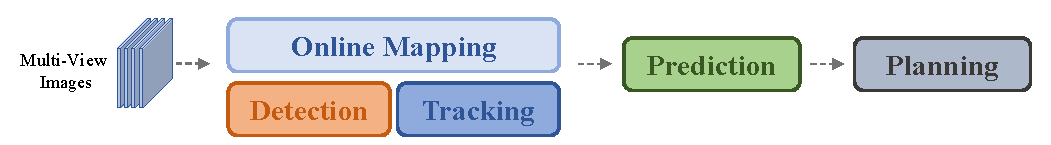
\includegraphics[width=1\linewidth]{Figures/Pipeline-a-Figure}
    \caption{传统自动驾驶范式}
    \label{fig:pipeline-a}
  \end{subfigure}
  \hfill
  \\
  \begin{subfigure}{1\linewidth}
    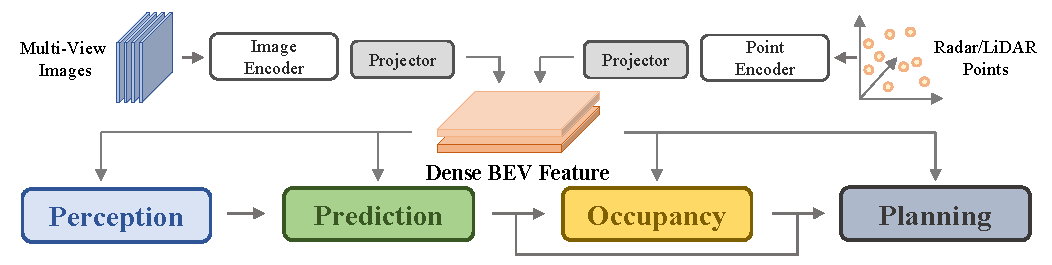
\includegraphics[width=1\linewidth]{Figures/Pipeline-b-Figure}
    \caption{密集BEV中心端到端范式}
    \label{fig:pipeline-b}
  \end{subfigure}
  \label{fig:short}
  \\
    \begin{subfigure}{1\linewidth}
    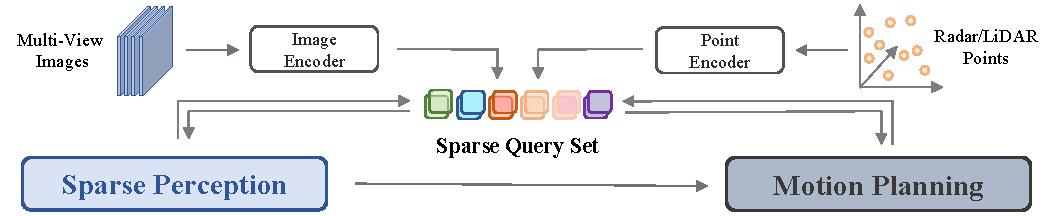
\includegraphics[width=1\linewidth]{Figures/Pipeline-c-Figure}
    \caption{稀疏查询中心端到端范式}
    \label{fig:pipeline-c}
  \end{subfigure}
  \hfill
  \end{subfigure}
  \begin{subfigure}{0.38\linewidth}
  \centering
    \begin{subfigure}{1\linewidth}
    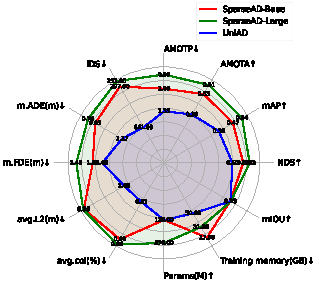
\includegraphics[width=1\linewidth]{Figures/RadarChart-Figure}
    \caption{本文方法与当前最优端到端自动驾驶方法\cite{hu2023planning}的综合性能对比}
    \label{fig:pipeline-d}
    \end{subfigure}
    \\
    \begin{subfigure}{1\linewidth}
    \end{subfigure}
    \\
    \begin{subfigure}{1\linewidth}
    \end{subfigure}

  \end{subfigure}

  \caption{主流自动驾驶范式对比。(a) 传统范式。(b) 密集BEV中心范式。(c) 本文提出的稀疏查询中心端到端自动驾驶范式。(d) (b)和(c)的代表性方法综合性能对比。}
  \label{fig:pipeline}
\end{figure}